\documentclass[draft,linenumbers]{agujournal}
\draftfalse
\usepackage{hyperref}
\usepackage[export]{adjustbox}
\addtolength{\oddsidemargin}{-.875in}
\addtolength{\evensidemargin}{-.875in}
	
\hypersetup{
    colorlinks=true,
    linkcolor=blue,
    filecolor=magenta,      
    urlcolor=cyan,
}

\journalname{Journal of Advances in Modeling Earth Systems (JAMES)}

\begin{document}


\nocite{*}
\bibliography{aguCLM5_bibtex}
\clearpage


\pagebreak
\begin{table}
\begin{center}
\begin{tabular}{ |c|c|c|c|c| } 
 \hline
 Parameter Name & Meaning & Units \\
  \hline
 slatop & Specific Leaf Area & m2/g \\ 
 froot\_leaf & Fine root:leaf ratio. & g/g \\
 stem\_leaf  & Stem:leaf ratio. & g/g \\ 
 n\_costs    & 6 parameters related to Nitrogen costs & g/g \\
 fracfixers  & Fraction of C available for fixation & - \\
  grperc  & Fraction of C used for growth respiration  & - \\
  leafcn  & Leaf C:N ratio. & g/g \\
     medlyn\_slope  & Slope of stomatal conductance curve & g/g \\
      lmr\_intercept & Intercept of leaf N /respiration relationship & \\
      frac\_ectomy\_fungi} & Fraction of active uptake that is ectohycorrhizal & - \\
      cn\_flex\_a & Parameter of N flexibility algorithm& \\
      cn\_flex\_b & Parameter of N flexibility algorithm & \\
      cn\_flex\_c & Parameter of N flexibility algorithm & \\
\hline
\end{tabular}
\end{center}
\caption{CLM5 Parameters subject to sensitivity analysis in this study. }
\label{table_parameters}
\end{table}


 \begin{table}
\begin{center}
\begin{tabular}{ |c|c|c|c|c| } 
 \hline
 Parameter Name & s1 &s2 & s3 & s4\\
  \hline
 slatop & 0.6761 & 0.8769 &1.2785 &1.4791\\ 
 froot\_leaf &  0.342 &0.671 &1.05 & 1.1\\
 stem\_leaf  &  0.3057 &0.61 &1 &1\\ 
 n\_costs    & 10$^{-2}$ &10$^{-2}$&  10$^{1}$& 10$^{2}$\\
 fracfixers  & 0 &0.5 & 2 & 4 \\
  grperc  &  0 & 0.5& 2 & 3\\
  leafcn  &0.7413 & 0.8932 & 1.1970  & 1.349\\
  
     medlyn\_slope  &0.5258 & 0.7191 & 1.1057  &1.29\\
      lmr\_intercept & 0.8539 & 0.9531 & 1.1512& 1.25\\
      frac\_ecto & 0 &0.5& 1 & 1 \\
      cn\_flex\_a &0 &0.5 & 2  &4\\
      cn\_flex\_b & 0.1 & 0.5 & 2  & 4\\
      cn\_flex\_c &0.001 & 0.1 & 10 & 100\\
\hline
\end{tabular}
\end{center}
\caption{Multipliers on the original values in CLM5 used in this sensitivity analysis .}
\label{table_ranges}
\end{table}



\begin{figure}[h]
    % \centering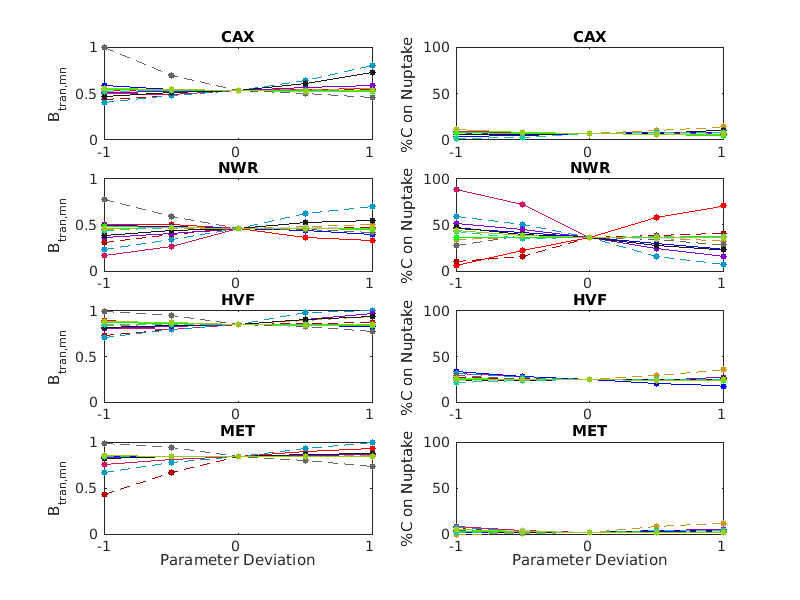
\includegraphics[width=0.5\textwidth, right]{lion-lo9
     \includegraphics[width=1.3\textwidth,left]{matlab/figures/btran_npp.png}
     \caption{Response of drought index ($B_{tran,mn}$) and the \% of NPP spent on Nitrogen uptake to parameter perturbation across -1 to +1 range of parameter variation at the Caxiuan\~a (CAX), Niwot Ridge (NWR), Harvard Forest (HVF) and Metolious MET) sites. Legend colours as for Figure \ref{NR1 state}}
     \label{btran state}
 \end{figure}
 
 \begin{figure}[h]
    % \centering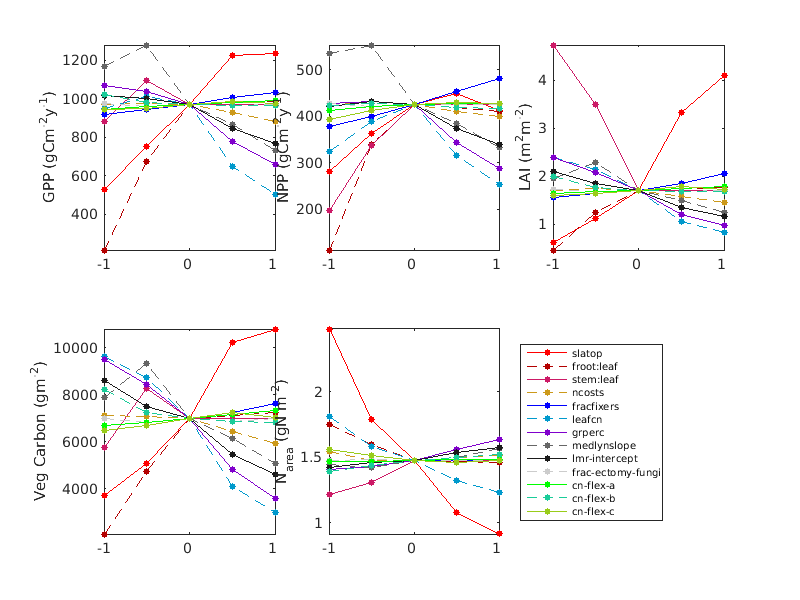
\includegraphics[width=0.5\textwidth, right]{lion-lo9
     \includegraphics[width=1.3\textwidth, left]{matlab/figures/NOVc_STATE_1CLM50defpft_trans_1x1pt_US-NR1_ens_MIC_y1_2012.png}
     \caption{Response of control model states and fluxes to parameter perturbation across -1 to +1 range of parameter variation (Table \ref{table_ranges}) at Niwot Ridge.}
     \label{NR1 state}
 \end{figure}
 
 
  \begin{figure}[h]
    % \centering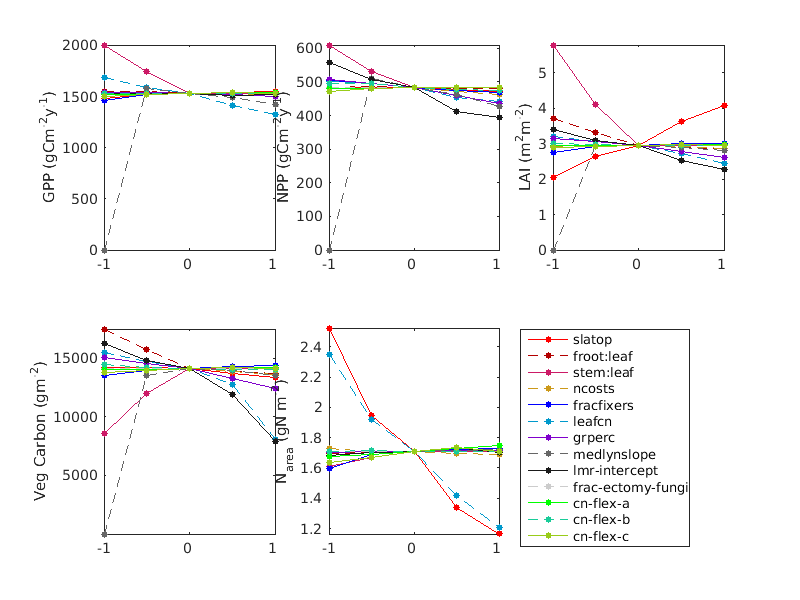
\includegraphics[width=0.5\textwidth, right]{lion-lo9
     \includegraphics[width=1.3\textwidth, left]{matlab/figures/NOVc_STATE_1CLM50defpft_trans_1x1pt_Br-cax_ens_MIC_y1_2012.png}
     \caption{Response of control model states and fluxes to parameter perturbation across -1 to +1 range of parameter variation (Table \ref{table_ranges}) at Caxiuan\~a National Forest}
     \label{CAX state}
  \end{figure}
  
 \begin{figure}[h]
    % \centering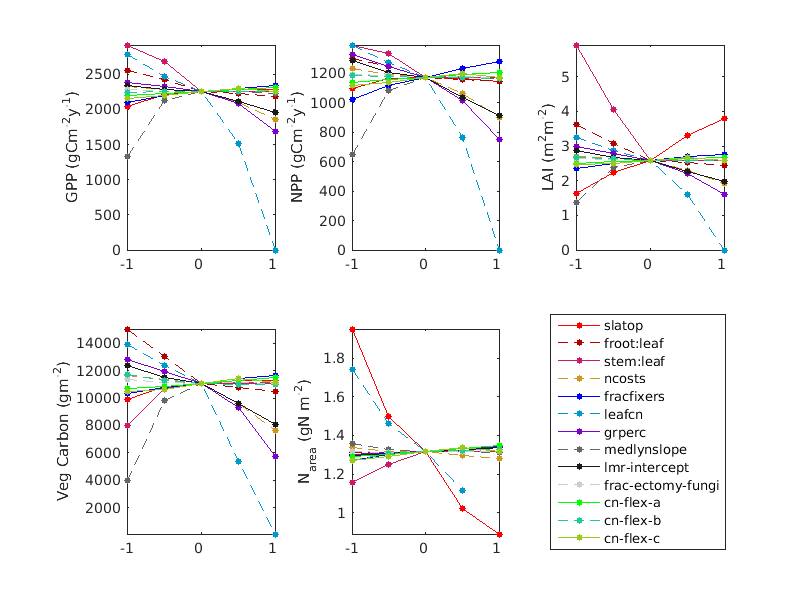
\includegraphics[width=0.5\textwidth, right]{lion-lo9
     \includegraphics[width=1.3\textwidth, left]{matlab/figures/NOVc_STATE_1CLM50defpft_trans_1x1pt_US_Ha1_ens_MIC_y1_2012.png}
     \caption{Response of control model states and fluxes to parameter perturbation across -1 to +1 range of parameter variation (Table \ref{table_ranges}) at Harvard Forest}
     \label{HVF state}
 \end{figure} 
  
 \begin{figure}[h]
    % \centering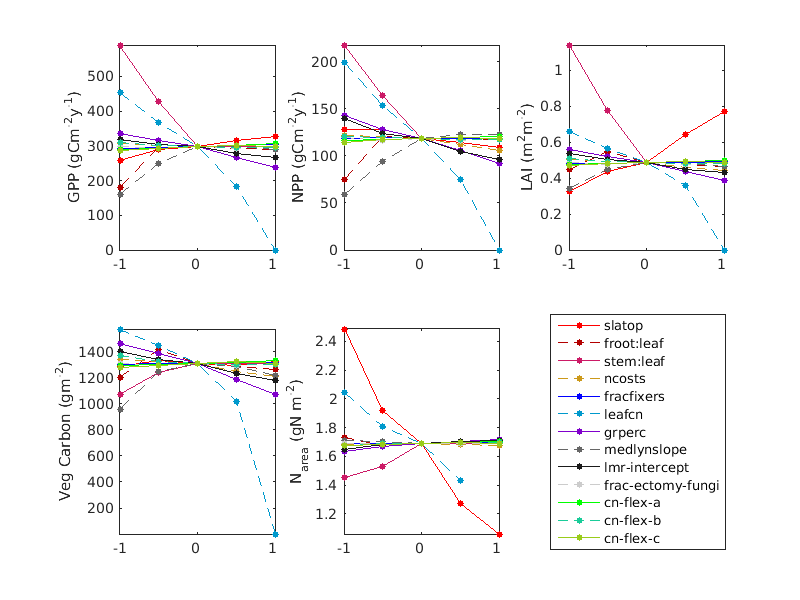
\includegraphics[width=0.5\textwidth, right]{lion-lo9
     \includegraphics[width=1.3\textwidth, left]{matlab/figures/NOVc_STATE_1CLM50defpft_trans_1x1pt_US-Me2_ens_MIC_y1_2012.png}
     \caption{Response of control model states and fluxes to parameter perturbation across -1 to +1 range of parameter variation (Table \ref{table_ranges}) at Metolius Forest}
     \label{MET state}
 \end{figure}
 
 
 
  \begin{figure}[h]
    % \centering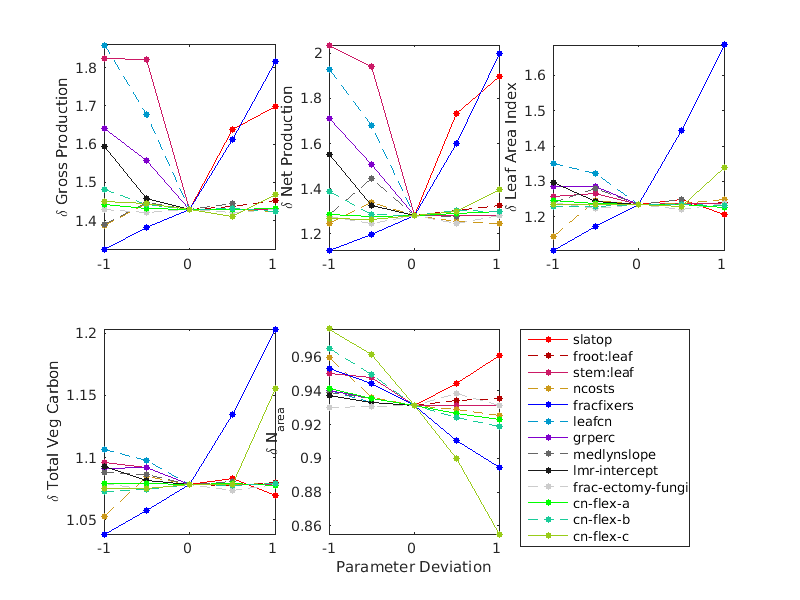
\includegraphics[width=0.5\textwidth, right]{lion-lo9
     \includegraphics[width=1.3\textwidth, left]{matlab/figures/NOVc_FERT_1CLM50defpft_celev_1x1pt_US-NR1_ens_MIC_p1_2012.png}
     \caption{Influence of parametric variation (over the range tested: -1 to +1, Table \ref{table_ranges}) on the model response (fertilized/control) to 15 years of CO$_{2}$ fertilization (550ppm) at Niwot Ridge}
     \label{NR1 celev}
  \end{figure}
  
  \begin{figure}[h]
    % \centering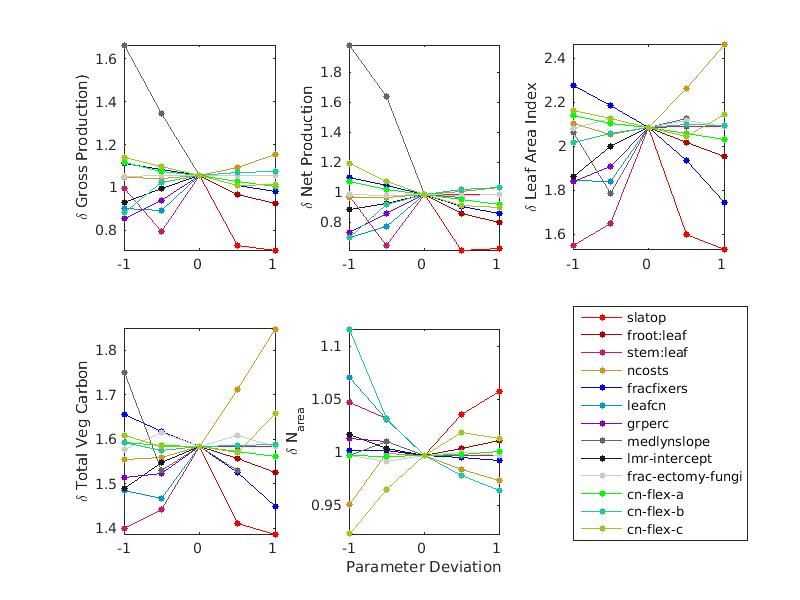
\includegraphics[width=0.5\textwidth, right]{lion-lo9
     \includegraphics[width=1.3\textwidth, left]{matlab/figures/NOVc_FERT_1CLM50defpft_ndep_1x1pt_US-NR1_ens_MIC_p1.png}
     \caption{Influence of parametric variation (over the range tested: -1 to +1, Table \ref{table_ranges}) on the model response (fertilized/control) to 15 years of Nitrogen fertilization (+5 kgN m$^{2}$ y$^{-1}$) at Niwot Ridge}
     \label{NR1 ndep}
  \end{figure}
  
      
 \begin{figure}[h]
     \centering
     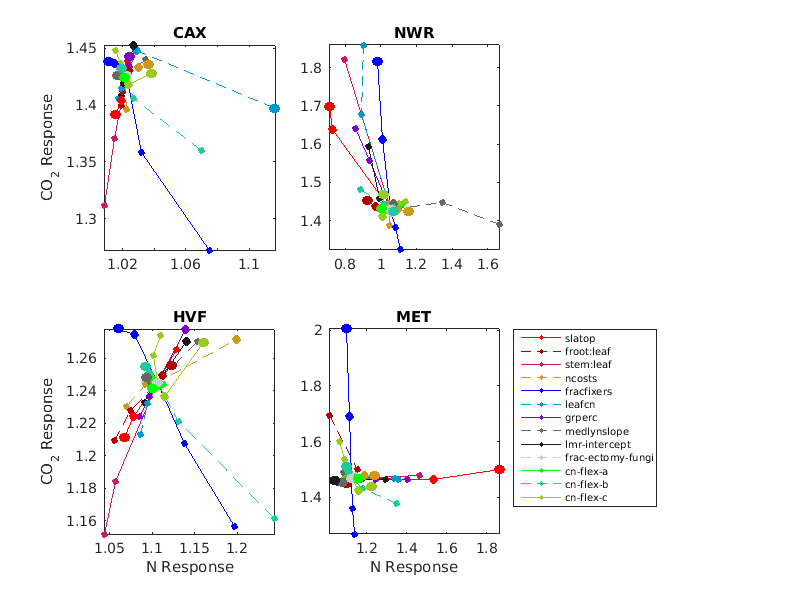
\includegraphics[width=1.55\textwidth, left]{matlab/figures/NOVc_CNdep_GPP1__p2012.png}
     \caption{Influence of parameteric variation on the model response (fertilized/control) to 15 years of CO$_{2}$ and N fertilization on gross primary productivity (GPP), across the Caxiuan\~a (CAX), Niwot Ridge (NWR), Harvard Forest (HVF) and Metolious MET) sites. }
     \label{GPP CO2 and N respones 2001}
  \end{figure}
  
 \begin{figure}[h]
     \centering
     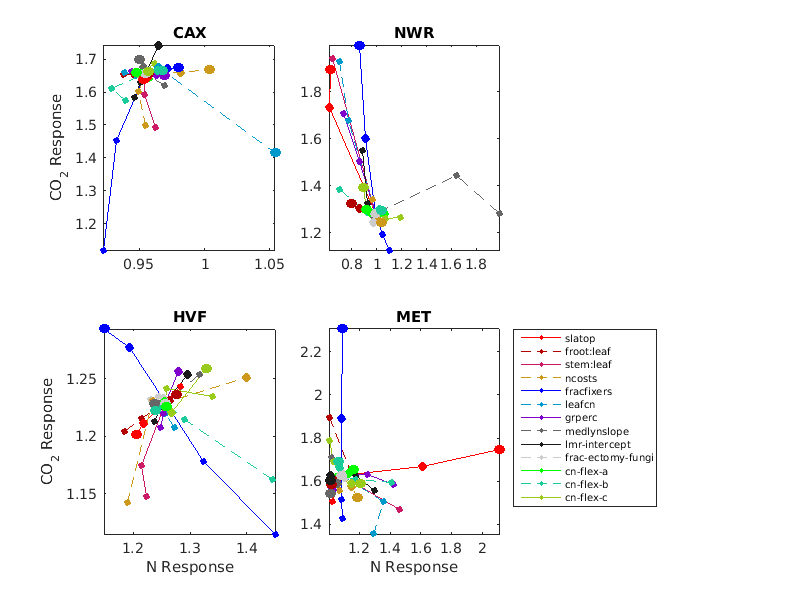
\includegraphics[width=1.55\textwidth, left]{matlab/figures/NOVc_CNdep_NPP1__p2012.png}
     \caption{Influence of parametric variation on the model response (fertilized/control) to 15 years of CO$_{2}$ and N fertilization on net primary productivity (NPP), across the Caxiuan\~a (CAX), Niwot Ridge (NWR), Harvard Forest (HVF) and Metolious MET) sites.}
     \label{NPP CO2 and N respones 2001}
  \end{figure}
  
  \begin{figure}[h]
     \centering
     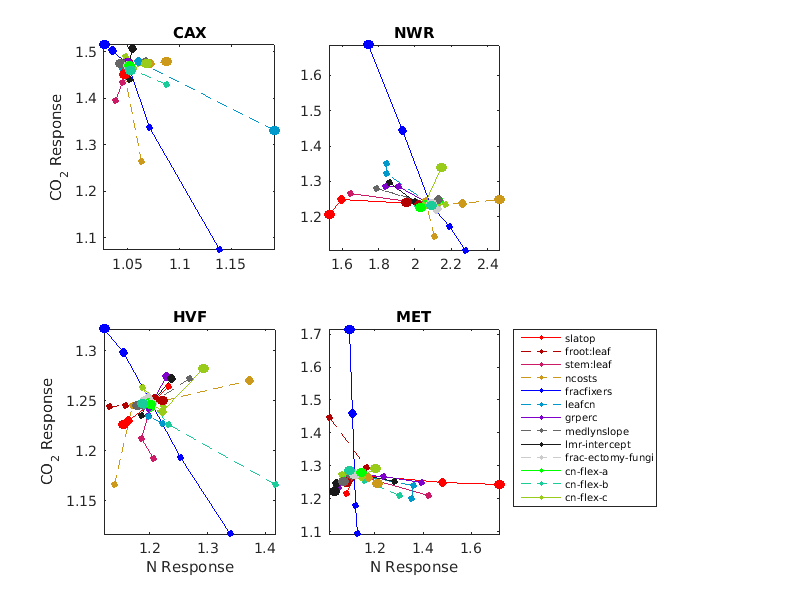
\includegraphics[width=1.55\textwidth, left]{matlab/figures/NOVc_CNdep_TLAI1__p2012.png}
     \caption{Influence of parametric variation on the model response (fertilized/control) to 15 years of CO$_{2}$ and N fertilization on leaf area index (LAI), across the Caxiuan\~a (CAX), Niwot Ridge (NWR), Harvard Forest (HVF) and Metolious MET) sites.}
     \label{LAI CO2 and N respones 2001}
  \end{figure}
  
 
    
 
\end{document}